\section{Unordered Delivery in MPEG-DASH}
\label{sec:transport}

MPEG-DASH is designed for an ordered transport protocol. Adapting it for an
unordered transport protocol requires several considerations. These
changes happen in two broad areas: the HTTP request and response semantics, and the rate
adaptation algorithms. We consider both of these in turn below.

\begin{figure}
  \centering
  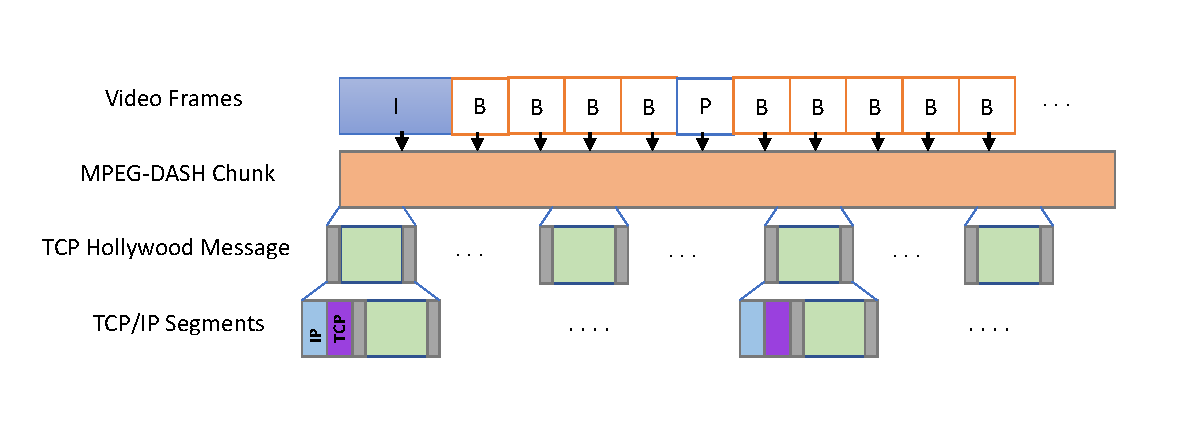
\includegraphics[width=\columnwidth]{figures/terminology2.pdf}
  \caption{Illustration of the terminology used in this paper and also the encapsulation of data for transport.}
  \label{fig:terminology}
\end{figure}

Given that our approach spans multiple layers of the stack, we must use carefully defined
terminology. The MPEG-DASH standard sends \emph{chunks}; these are groups of video
\emph{frames} that have the same duration. In our approach, the server will send these
using TCP Hollywood \emph{messages}. A chunk may be split across more than one message,
but a message will never contain data from more than one chunk. Finally, messages are
send in TCP \emph{segments}; a segment may contain data from more than one message, and
may contain only some of the data for a message.
Figure \ref{fig:terminology} illustrates this terminology.

\subsection{HTTP Request/Response Semantics}

As discussed in the previous section, the transmission unit of TCP Hollywood is a message:
complete messages are delivered to the application when they arrive. Care must be taken in
deciding what should be sent in each message: if a message is too large, then its loss
will have a greater impact on the application's quality-of-experience; too small, and the
ratio of payload to header will be low. Sending an entire chunk per message means that,
in the event a segment that makes up the message is lost, upwards of 1 second of video
data is not delivered to the application. Sending a single video frame is the
other extreme: we minimise the impact of loss on QoE, but reduce the efficiency of our
application, by sending a TCP/IP header per video frame. As a result, we opt for a
compromise: we send fixed-size (1400 byte) messages. This reduces the impact of loss 
(though not minimally), while amortising the header across a larger payload.

TCP Hollywood supports multi-streaming over a single TCP connection, allowing for the
separation of the control and data channels. We use separate streams for HTTP request and
response headers, sending each as separate TCP Hollywood messages. This allows the client
to request later chunks while earlier chunks are still downloading. The server still sends
chunks sequentially, but does not have to wait for the next request to arrive; this is
especially useful in high latency networks. Figure \ref{fig:hollywood_download}
illustrates chunk retrieval with HTTP over both standard TCP and TCP Hollywood.

Our use of multi-streaming in TCP Hollywood is similar to HTTP/1.1 pipelining and bundle
requests in HLS \cite{muller2012evaluation}. However, these approaches require quality
estimates to be submitted for all chunks at request time. This means that a quality
estimate may be two or more chunk durations old before being used at the server.
Fluctuations in network conditions in the interval between request and response mean that
these quality estimates can be incorrect. Under TCP Hollywood, requests can be sent while
chunks are downloading, allowing for the server to receive a more recent and accurate
estimate of network conditions. This reduces the likelihood of an under or over estimation
of performance, improving quality-of-experience. Further, HTTP/1.1 pipelining suffers
from transport-layer head-of-line blocking in standard TCP, which is eliminated under TCP Hollywood.

Finally, TCP Hollywood can discard late messages and continue play-out,
thereby limiting stall events only to those cases when the play-out buffer is completely
empty.

\begin{figure}
    \centering
    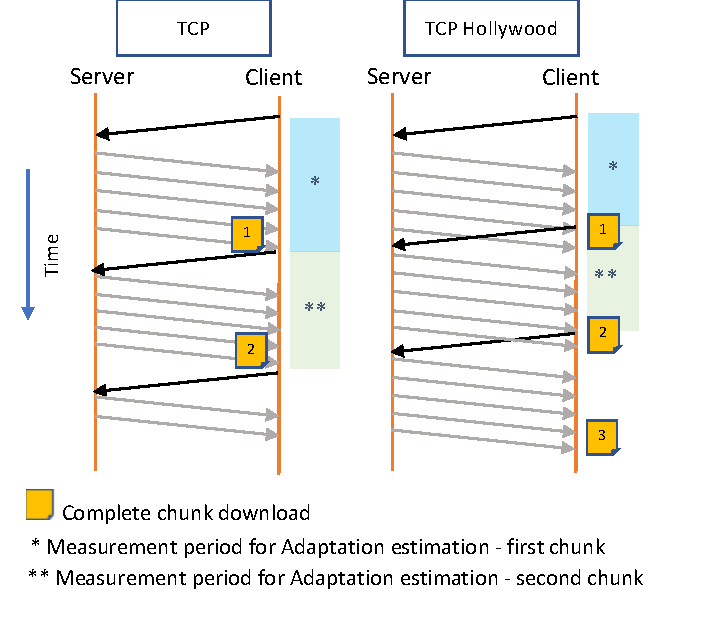
\includegraphics[width=\columnwidth]{figures/tcph-download.pdf}
    \caption{An illustration of chunk download with HTTP over TCP and over TCP Hollywood. The shaded area represents the measurement period for each chunk. }
    \label{fig:hollywood_download}
\end{figure}

The requested chunks of video are transmitted on a single stream, using fixed size
messages. As the server is content-agnostic, it is unable to set an expiry time for messages, and
all messages are sent reliably. A content-aware server would set this to the relative presentation time of the chunk.
For the sake of simplicity, audio
stream is not used. Each message is appended with a monotonically increasing sequence
number and a stream offset. The stream offset is the offset of the last byte of the
message within this stream, where a stream includes all chunks that have been transmitted
previously. Both fields are used by the receiver to reorder the messages and detect
losses. We expanded the function of the play-out buffer to include de-jittering and
reordering of the incoming messages.

The commonly used ISO Base Media File Format (MP4) is not suitable for TCP Hollywood due to its lack of tolerance for packet losses. Hence, we use MPEG Transport streams (TS), which are allowed as part of the MPEG-DASH standard and also used in HLS.

\subsection{Rate Adaptation Algorithms}

Performance of a MPEG-DASH system relies heavily on a good rate adaptation algorithm.
Such algorithms use application-level measurements such as buffer length, throughput, time to
download a chunk, or a combination of these to select an appropriate quality for
download \cite{beben2016abma+, spiteri2016bola, li2014probe}. There is some consensus
among researchers that buffer-based algorithms are more performant and reliable in a wider
variety of network conditions than other algorithms 
\cite{huang2015buffer, karagkioules2017comparative}.

Our TCP Hollywood-based MPEG-DASH client uses the open-source BOLA 
(Buffer Occupancy based Lyapunov Algorithm) rate adaptation algorithm \cite{spiteri2016bola} adapted from the MPEG-DASH reference
client implementation, dash.js.\footnote{\url{https://github.com/Dash-Industry-Forum/dash.js/wiki}}
BOLA uses the amount of video currently buffered to calculate the quality level (bit-rate
level) for the next chunk. For live video, where buffer sizes are limited, the algorithm's implementation 
uses throughput estimates to further reduce over-estimation and stalling, and an effective buffer level to prevent under-estimation. In the event that the buffered duration is not limited by network conditions but by the availability of the next chunk at the server (e.g., it has not been captured yet) or the size of the play-out buffer, the effective buffer level is used by the client to request higher quality chunks even when the actual buffered duration is low. The effective buffer level is determined by the time spent waiting before downloading the next chunk. Algorithm \ref{algo:tcp_dash} shows the operation of rate adaptation using BOLA in a typical TCP based DASH client. Note that the quality estimation logic of the BOLA algorithm was adapted from dash.js without any modifications and remains unchanged even for TCP Hollywood, hence we do not further explain the inner workings of the estimation process. 


\begin{algorithm}[t!]
	\begin{algorithmic}[1]
   		\Procedure{DownloadStream}{}
		\State $\textit{n} \gets \textit{index of current chunk}$
		\State $N \gets \textit{Total number of chunks}$
		\State $B \gets \textit{Maximum Buffer Length}$
		\State $b_{now} \gets \textit{Current Buffer Length}$
		\State $b_{e} \gets \textit{Effective Buffer Level}$
		\State $S_n^q \gets \textit{Size of chunk with index n and quality q}$
		\State $B_n^q  \gets \textit{Bytes received for chunk with index n and quality q }$
		\State $Rx_T \gets Minimum Receive Threshold$
		\While {$\text{n} < \text{N}$}
			\If {$b_{now} > B$}
				\State $\Delta t \gets B - b_{now}$
				\State $WaitForDuration (\Delta t)$
			\EndIf
			\State $b_{e} \gets b_{e} + \Delta t$
			\State ${q \gets GetBolaQualityEstimate(b_{now},  b_{e})}$
			\State ${DownloadChunk(q, n)}$
		\EndWhile
		\EndProcedure
	\end{algorithmic}
	\caption{BOLA rate adaptation under TCP}
    	\label{algo:tcp_dash}
\end{algorithm}

In the presence of packet loss and duplication, that is possible with TCP Hollywood, the calculation 
mechanisms for measurements have to be modified. BOLA algorithm is written for standard TCP, where HoL blocking means that the client must wait for all data to arrive. In TCP Hollywood, HoL blocking is eliminated, allowing the client to continue if even some data hasn't arrived. Therefore, we introduce a new parameter, $Rx_{T}$, the Receive Threshold: when the ratio of the bytes received in a chunk reaches $Rx_{T}$, the client continues with its rate adaptation as if the entire chunk had arrived. Care is needed when selecting the value of RxT: if it is too low, the rate adaptation will be performed on a partial view of network conditions, which may result in selecting an unsuitable rate; picking RxT too high would diminish the impact of eliminating HoL blocking. After experimenting with a range of RxT values between 0.75 and 0.99, under stable network conditions, we chose 0.9. We found this value was sufficiently high to include the current chunk as part of the buffered duration (only 10\% of the chunk remains to be downloaded, with some data in-flight, and a limited number of messages that may delayed and subsequently discarded by TCP Hollywood if they miss their deadline), and gather measurements for the next chunk, while sufficiently low as to enable the benefits of TCP Hollywood. While our experiments only considered 1 second chunks, we expect this value to hold for other chunk durations. The modified operation for TCP Hollywood is shown as Algorithm \ref{algo:tcph_dash}. Note that any throughput estimations used by the BOLA algorithm, while not shown as part of the pseudocode, will also use only the partial download of the chunk. 

\begin{algorithm}
	\begin{algorithmic}[1]
   		\Procedure{DownloadStream}{}
		\State $\textit{n} \gets \textit{index of current chunk}$
		\State $N \gets \textit{Total number of chunks}$
		\State $B \gets \textit{Maximum Buffer Length}$
		\State $b_{now} \gets \textit{Current Buffer Length}$
		\State $b_{e} \gets \textit{Effective Buffer Level}$
		\State $S_n^q \gets \textit{Size of chunk with index n and quality q}$
		\State $B_n^q  \gets \textit{Bytes received for chunk with index n and quality q }$
		\State $Rx_T \gets Minimum Receive Threshold$
		\State $L \gets Losses since last download$
		\While {$\text{n} < \text{N}$}
			\If {$b_{now} > B$}
				\State $\Delta t \gets B - b_{now}$
				\State $WaitForDuration (\Delta t)$
			\EndIf
			\State $b_{e} \gets b_{e} + \Delta t$
			\If {$L > 0$}
				\State $b_{e} \gets b_{e} - ChunkDuration$
			\EndIf
			\State ${q \gets GetBolaQualityEstimate(b_{now},  b_{e})}$		
			\State $InitiateChunkDownload(q, n)$
			\State $WaitUntil (B_n^q < Rx_T * S_n^q)$
		\EndWhile
		\EndProcedure
	\end{algorithmic}
	\caption{BOLA rate adaptation under TCP Hollywood}
	\label{algo:tcph_dash}
\end{algorithm}

The $Rx_{T}$ parameter can be used with other adaptation algorithms as it impacts only the measurements and not the quality estimation. Preliminary testing for this study was carried out using both the buffer-based BOLA algorithm and the throughput-based PANDA algorithm \cite{li2014probe}. Generally, we found BOLA outperformed PANDA for standard TCP and TCP Hollywood, in terms of stall avoidance and bit rate switching, a finding confirmed by previous studies \cite{karagkioules2017comparative}. Note that the main advantages of TCP Hollywood (shown in Figure \ref{fig:hollywood_download}) are the removal of head-of-line (HoL) blocking, and the addition of chunk request pipelining and these remain regardless of the algorithm used. 
